\documentclass[10pt,twocolumn,letterpaper]{article}

\usepackage{iccv}
\usepackage{times}
\usepackage{epsfig}
\usepackage{graphicx}
\usepackage{amsmath}
\usepackage{amssymb}

% Include other packages here, before hyperref.

% If you comment hyperref and then uncomment it, you should delete
% egpaper.aux before re-running latex.  (Or just hit 'q' on the first latex
% run, let it finish, and you should be clear).
\usepackage[pagebackref=true,breaklinks=true,letterpaper=true,colorlinks,bookmarks=false]{hyperref}

 \iccvfinalcopy % *** Uncomment this line for the final submission

% Pages are numbered in submission mode, and unnumbered in camera-ready
\ificcvfinal\pagestyle{empty}\fi

\begin{document}

%%%%%%%%% TITLE
\title{CAP 5516 Medical Image Computing Spring 2022 Project Report}

\author{Kyle Beggs\\
Department of Mechanical and Aerospace Engineering\\ 
University of Central Florida\\
{\tt\small kbeggs07@knights.ucf.edu}}

\maketitle
% Remove page # from the first page of camera-ready.
\ificcvfinal\thispagestyle{empty}\fi


\begin{abstract}
    1D models of the cardiovascular system are useful for surgical planning where time is of the essence due to their much reduced computational cost. These models are built form extracting the centerlines from 3D geometry. It is important for centerline extraction to not miss any branches as this can impact results and having a fully automated pipeline for simulation which includes centerline extraction is an attractive feature. State-of-the-art centerline extraction methods require user input and fail to capture branches often. This project seeks to further improve upon current approaches using Neural Networks for centerline extraction.
\end{abstract}


%%%%%%%%%%%%%%%%%%%%%%%%%%%%%%%%%%%%%%%%%%%%%%%%%%%%%%%%%%%%%%%%%%%%%%%%%%%%%%%%%%%%%%%%%%
\section{Problem Definition}

In recent years there has been significant interest in developing a pipeline for cardiovascular surgical planning for patient-specific care via 3D Computational Fluid Dynamics (CFD) simulations \cite{morrisonAdvancingRegulatoryScience2018}. The main barrier to the implementation of such a tool for surgeons to use is computational cost, despite sustained advancements in compute power. However, the success of many proposed surgeries such as coronary bypasses depends on macro-hemodynamic quantities that can be accurately simulated with 1D models effectively reducing the computational cost by a factor of hundreds compared to 3D. An equally important goal in building a pipeline for patient-specific cardiovascular surgical planning is to be fully automated. Recent research thrust in this direction aims for these goals but requires user input \cite{pfallerAutomatedGeneration0D2021}.
 
Centerline extraction can be performed via the grassfire or shrinking ball algorithms with no user input, but these often fail to achieve the robustness needed for the results to be directly used in simulation. They often have unphysiologically small vessel branches near bifurcations and struggle where there might be sudden widening or narrowing of vessels, which is common in diseased patients. Other approaches simulate a wave front by solving the Eikonal equation or compute a minimum cost path, however, these require input of a seed and/or target outputs \cite{antigaCenterlineComputationGeometric2003} \cite{jinRobustEfficientCurve2016}.

In light of this, the goal of this project is to improve upon the current state of the art neural networks to segment the centerline of the vessel is desirable such that no user input is required and no further pre-processing is needed before performing 1D surgical planning simulations.


%%%%%%%%%%%%%%%%%%%%%%%%%%%%%%%%%%%%%%%%%%%%%%%%%%%%%%%%%%%%%%%%%%%%%%%%%%%%%%%%%%%%%%%%%%
\section{Related Work}

The first attempt at extracting centerlines (at least claimed by the authors) was by Guo et al. who used a Fully Convolutional Network for extracting coronary artery centerlines \cite{guoDeepCenterlineMultitaskFully2019}. Lenga et al. built a system to extract centerlines on rib bones using the feature map output from the network to perform an external extraction algorithm \cite{lengaDeepLearningBased2019}. Although technically not using Deep Learning to output centerlines, it is included because it is fully-automated and that is a goal of this project. The next deep learning approach to extracting centerlines is DeepVesselNet where they attempt to segment the geometry, centerline, and bifurcation points \cite{tettehDeepVesselNetVesselSegmentation2020}. They use a cross-hair filter for speeding up computation and introduce a new loss function based on cross-entropy but takes into account the high class imbalance as centerlines represent a very small fraction (< 3\%) of the total pixels in an image. They also use angiogenesis models to generate synthetic data to train on since obtaining 3D vascular datasets along with centerline labels are nonexistent. The most recent attempt by Mostafa et al. first identifies a seed point and then narrows the input image to a CNN to the local area around that point. The output of the CNN is the next point on the centerline, which then becomes the new local area input into the CNN \cite{mostafaImprovedCenterlineExtraction2021} - similar to the wave front technique pioneered by Antiga et al.

\section{Methods}

Due to the lack of cardiovascular datasets freely available, the only two datasets found are used. A synthetic dataset from the DeepVesselNet paper and a real dataset from the Vascular Model Repository \cite{wilsonVascularModelRepository2013}. The DeepVesselNet synthetic dataset has 136 images of size (325, 304, 600) and will be useful in testing the robustness of the network as it has a large amount of bifurcations and variance in vessel size. A sample of the dataset is shown in .

\begin{figure}[!h]
    \begin{center}
       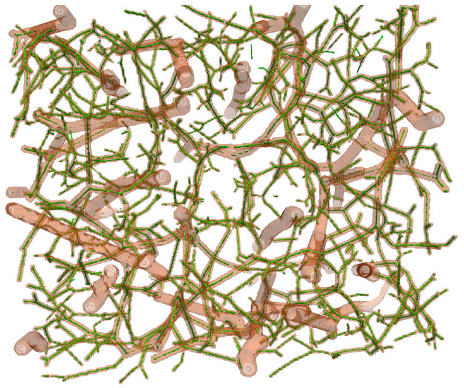
\includegraphics[width=0.95\linewidth]{figures/dataset-deepvesselnet.png}
    \end{center}
       \caption{Example segmentation and centerline.}
    \label{fig:dataset example}
\end{figure}

An architecture similar to that of Guo et al. \cite{guoDeepCenterlineMultitaskFully2019} is used where segmentations (inputs) and distance maps (targets) are generated using the DeepVesselNet dataset. The distance maps are generated from the supplied centerlines as 1-pixel wide `lines'. The input to the network is the segmentation and output is a centerline distance map. This approach is used because complex and well performing segmentation networks exists, and so we want to begin from that point. The method should also be generalizable as its approach to finding branch endpoints does not rely on detecting particular anatomical features as in \cite{mostafaImprovedCenterlineExtraction2021}. Endpoints are needed in the minimal path algorithm for final output of the centerline but represent a tiny fraction of the total voxels, suffering from major class imbalance. Guo et al. remedies this problem by generating a confidence map around the endpoint using a Gaussian distribution.

Two objectives will be investigated:
\begin{enumerate}
    \item The use of strided convolutions vs pooling operations in the encoder part of the network.
    \item What is the effect of training with perfect ground truth centerlines over truths generated with current state-of-the-art methods?
\end{enumerate}

Objective two is a continuation of a question posed at the conclusion of Guo et al. because they generated the truth centerlines using current state-of-the-art methods (termed `baseline') and then compared their network to those same baselines. Despite the conundrum of this approach, they still found their method was able to generalize better and increased accuracy of 30\%! They propose using the better output from their method to then train a second network and perhaps achieve even higher accuracies. Metrics that will be used to assess final performance: mean centerline to centerline distance, Hausdorff distance, and overall success rate which is defined determines that the centerline covers all branches sufficiently, has no spurious false positive branch, no wrong bifurcation, and no obvious deviation from the center throughout all sections.

\begin{figure}[!h]
\begin{center}
   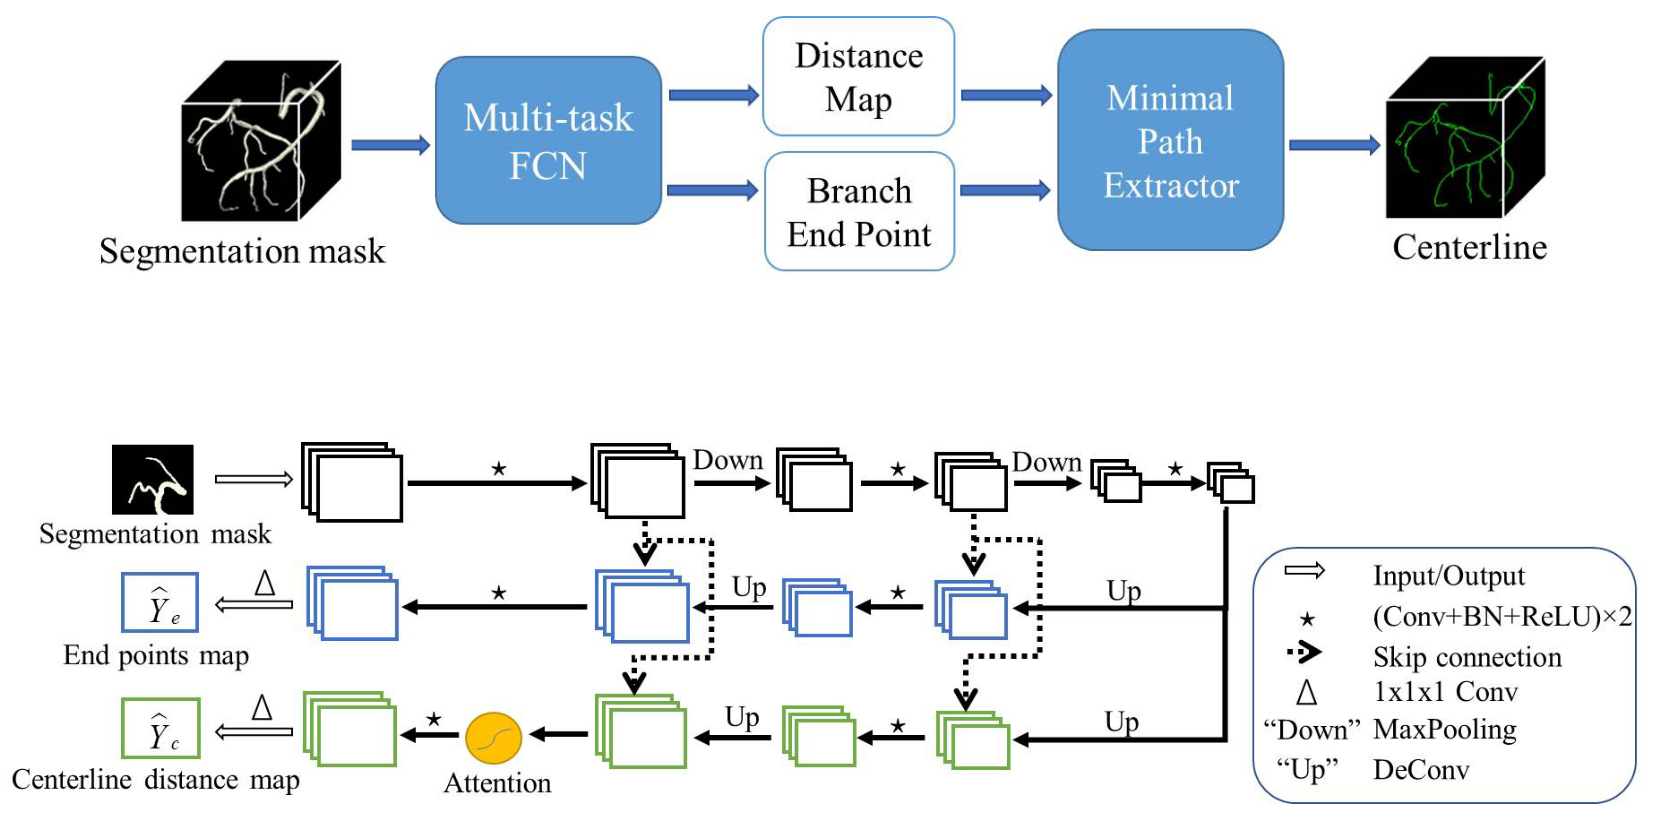
\includegraphics[width=0.95\linewidth]{figures/network-arch-guo.png}
\end{center}
   \caption{Network architecture used by Guo et al. \cite{guoDeepCenterlineMultitaskFully2019} and the base for this work.}
\label{fig:fig1}
\end{figure}

In this work, only the centerline maps are output and compared which should suffice for the objectives at hand. The centerline distance maps are generated via the binary distance transform which measures the distance from a pixel with 0 to a pixel with a 1. The $\log()$ transform is then computed of the map to further highlight the centerline. The final map along with the centerline is shown in \ref{fig:centerline map}.

\begin{figure}[!h]
    \begin{center}
       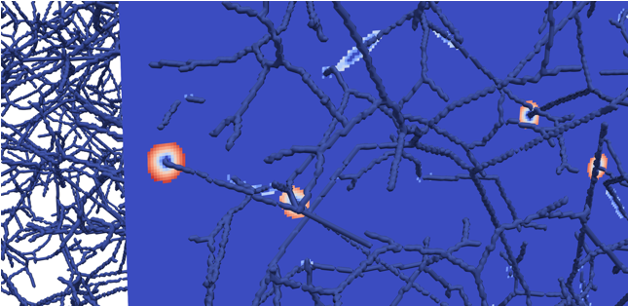
\includegraphics[width=0.95\linewidth]{figures/map-centerline.png}
    \end{center}
       \caption{Centerline and centerline distance map.}
    \label{fig:centerline map}
\end{figure}

The inputs images are randomly flipped among each axis and randomly cropped to a size of (300, 300, 300). The ADAM optimizer is used on a Mean Squared Error loss function with a Cosine Annealing Learning Rate Scheduler. The scheduler begins with a learning rate of 1e-3 and the batch size is 6 and the model is trained for 100 epochs. It should be noted that the code for \cite{guoDeepCenterlineMultitaskFully2019} was not provided and so the model was pieced together beginning from a Residual UNet based code.



%%%%%%%%%%%%%%%%%%%%%%%%%%%%%%%%%%%%%%%%%%%%%%%%%%%%%%%%%%%%%%%%%%%%%%%%%%%%%%%%%%%%%%%%%%
\section{Results}

Unfortunately due to much time spent on initial debugging issues, only objective 1 was able to be investigated. Four models were compared - pooling, pooling with residual connections, striding, striding with residual connections. The training and validation loss data are presented in figure \ref{fig:losses} and table \ref{table:results}.

\begin{table}
\begin{center}
\begin{tabular}{ c | c | c | c }
\hline
Method & Train Loss & Val Loss & Time (hr) \\
\hline
Pooling & 1.75e-3 & 1.75e-3 & 1.32 \\
Striding & 1.08e-3 & 1.07e-3 & 1.57 \\
Pooling w/ Res. & \bf 1.41e-4 & \bf 1.15e-4 & 1.33 \\
Striding w/ Res. & 5.54e-4 & 5.21e-4 & \bf 1.31 \\
\hline
\end{tabular}
\end{center}
\caption{Results for your milestone and final reports.}
\label{table:results}
\end{table}

\begin{figure}[!h]
    \begin{center}
       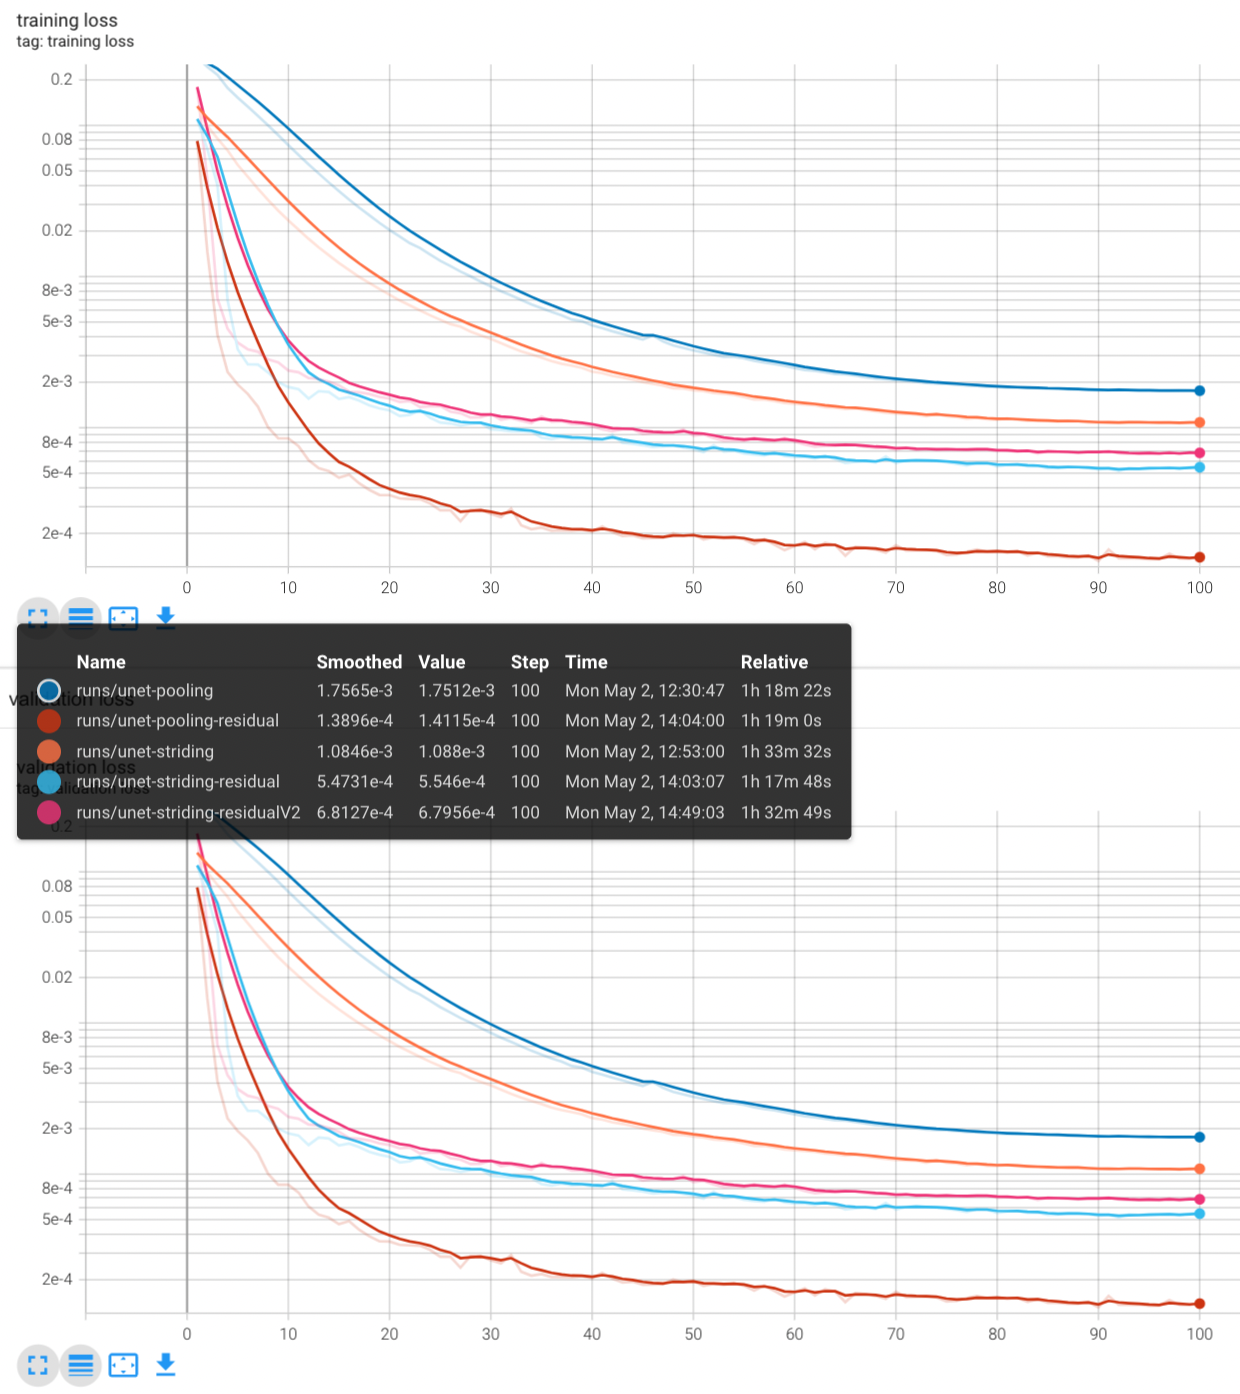
\includegraphics[width=0.95\linewidth]{figures/losses.png}
    \end{center}
       \caption{Training and validation loss curves.}
    \label{fig:losses}
\end{figure}


Interestingly, when pooling operations are replaced with striding using a plain UNet (\emph{no residual connections}) the striding improves performance, yet when residual connections are added, pooling is better. The target distance map is seen in figure \ref{fig:target} and the trained network outputs using pooling and striding can be seen in figures \ref{fig:output pooling} and \ref{fig:output striding}, respectively. It can be seen that the pooling does a slightly better job of localizing the centerline.

\begin{figure}[!h]
    \begin{center}
       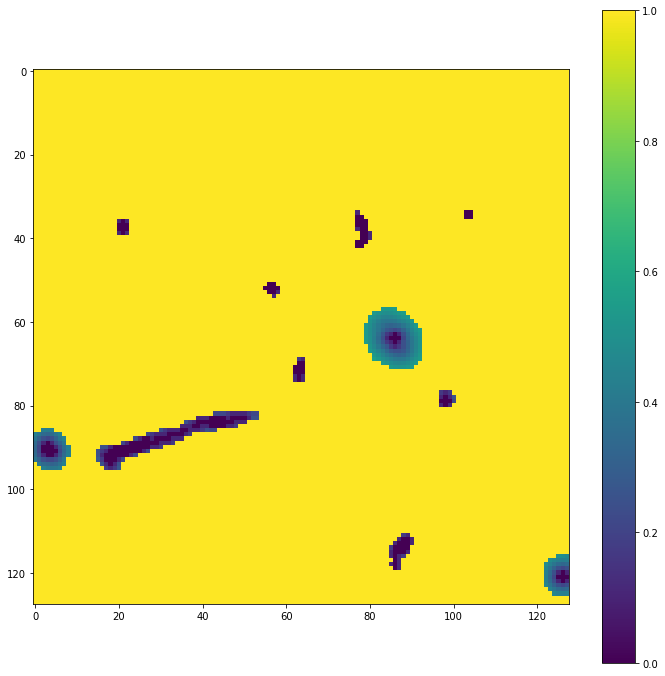
\includegraphics[width=0.95\linewidth]{figures/output-target.png}
    \end{center}
       \caption{Target centerline distance map.}
    \label{fig:target}
\end{figure}

\begin{figure}[!h]
    \begin{center}
       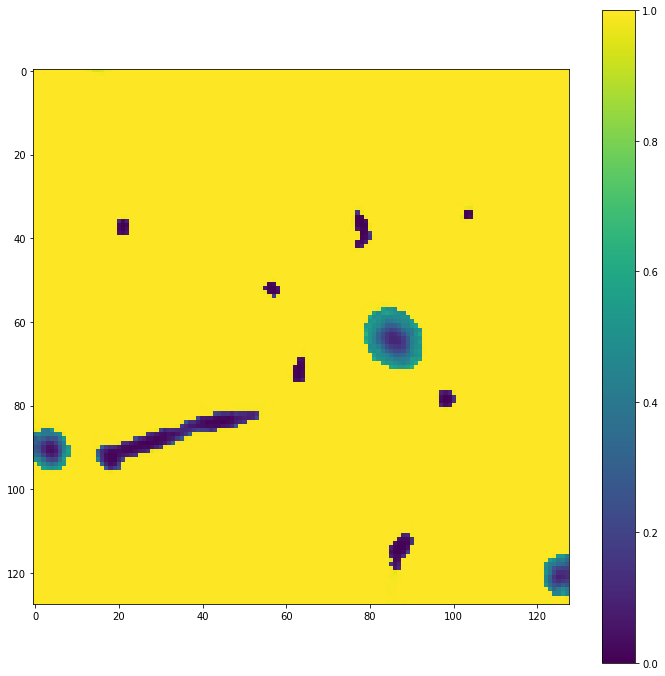
\includegraphics[width=0.95\linewidth]{figures/output-pooling-residual.png}
    \end{center}
       \caption{Network output using pooling with residual connections.}
    \label{fig:output pooling}
\end{figure}

\begin{figure}[!h]
    \begin{center}
       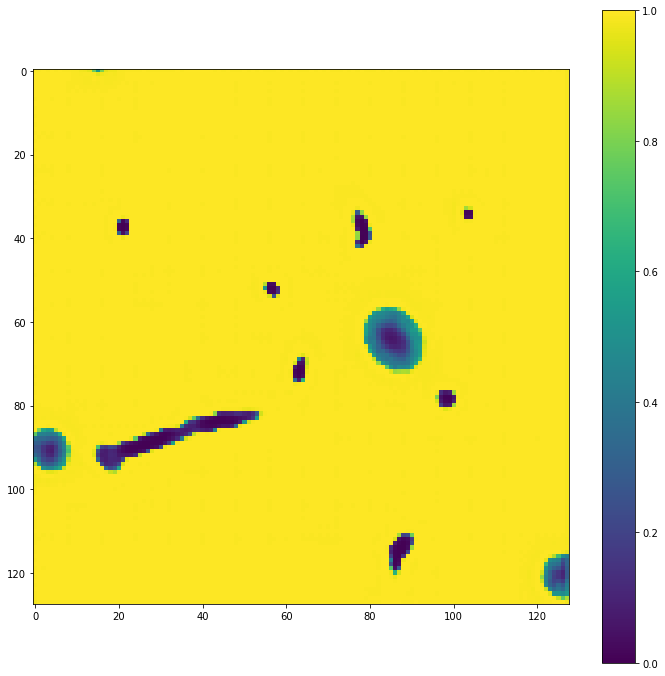
\includegraphics[width=0.95\linewidth]{figures/output-striding-residual.png}
    \end{center}
       \caption{Network output using striding with residual connections.}
    \label{fig:output striding}
\end{figure}


%%%%%%%%%%%%%%%%%%%%%%%%%%%%%%%%%%%%%%%%%%%%%%%%%%%%%%%%%%%%%%%%%%%%%%%%%%%%%%%%%%%%%%%%%%
\section{Conclusion}

Unfortunately not much discussion is available due to limited results, but the pooling vs striding operations switching which performs better when residual connections are added is something interesting and should be investigated further.


{\small
\bibliography{centerline_bifurcation}
\bibliographystyle{IEEEtran}
}

\end{document}
